% tempalte.tex
% Author: 傅申
% 本文件是 实验报告模板.docx 与 实验报告模板.tex 的衍生作品,其著作权属于中国科学技术大学计算机实验教学中心.

% 本文件可使用TeXLive发行版(作者使用的是TeXLive 2021,但理论上2016及以后均可)的xelatex命令编译.
\documentclass[UTF8,fontset=fandol]{ctexart}
\usepackage{LabReport}
\usepackage{hyperref}
\hypersetup{
    colorlinks=true,
    linkcolor=black,
    filecolor=blue,      
    urlcolor=blue,
    citecolor=cyan,
}
\usepackage{makecell}
\begin{document}
\maketitle{综合实验}
\section*{实验目的}
%列举本实验的实验目的,除指导书上列出的之外,鼓励自行总结及扩展。
\begin{itemize}
  \item 熟练掌握前面实验中的所有知识点
  \item 熟悉几种常用通信接口的工作原理及使用
  \item 独立完成具有一定规模的功能电路设计
\end{itemize}
\section*{实验环境}
%列举本实验所用到的各种软硬件环境,如EDA工具、实验平台、实验设备等。
\begin{itemize}
  \item Windows PC
  \item Microsoft Visual Studio Code
  \item Xilinx Design Tools Vivado HL Design Edition 2019.1 
  \item \href{http://fpgaol.ustc.edu.cn}{FPGAOL}
\end{itemize}
\section*{实验练习}
%如无特殊说明,则应完成对应实验手册上的所有练习题目,将过程和结果以图文并茂的形式体现在本报告中,建议实验过程中随手保存各种截图。
在 FPGAOL 平台上实现了一个简单的 LC-3 片上系统, 并且能正确运行示例程序, 但是没有通过串口进行交互式操作.
\subsection*{LC-3 简介}
LC-3 (Little Computer 3) 是一个图灵完备的 16 位计算机, 拥有 $2^{16}\times16$ bits 的内存, 8 个 16 位寄存器和若干个系统寄存器 (如 PC, IR, Condition Codes, etc.). 
它拥有包含 15 条指令的指令集, 每条指令的操作码为指令的高 4 位. 具体的指令集如图 \ref{Fig:isa} 和表 \ref{Tab:isa}, 其中带有上标$^+$的指令会修改条件码寄存器.
\img{.8}{images/isa.pdf}{LC-3 的指令集}{Fig:isa}
\begin{table}[!htbp]
  \centering
  \caption{LC-3 的指令集}
  \label{Tab:isa}
  \begin{tabular}{cccc}
    \toprule 
    指令名 & 指令全称 & 操作码 & 操作 \\
    \midrule
    ADD$^+$ & Addition & 0001 & \makecell{\texttt{DR = SR1 + SR2} \\ 或 \texttt{DR = SR1 + imm5}} \\
    \midrule
    AND$^+$ & Bit-Wise Logical AND & 0101 & \makecell{\texttt{DR = SR1 \& SR2} \\ 或 \texttt{DR = SR1 \& imm5}} \\
    \midrule
    BR  & Conditional Branch & 0000 & \makecell{\texttt{if (nzp \& cond\_code)} \\\texttt{PC = PC + PCoffset9}} \\
    \midrule
    JMP & Jump & 1100 & \texttt{PC = BaseR} \\
    \midrule
    JSR & Jump to Subroutine & 0100 & \makecell{\texttt{Temp = RC}\\\texttt{PC = BaseR} \\或 \texttt{PC = PC + offset11}\\\texttt{R7 = Temp}}  \\
    \midrule
    LD$^+$  & Load & 0010 & \texttt{DR = mem[PC + PCoffset9]} \\
    \midrule
    LDI$^+$ & Load Indirect & 1010 & \texttt{DR = mem[mem[PC + PCoffset9]]} \\
    \midrule
    LDR$^+$ & Load Base+Offset & 0110 & \texttt{DR = mem[BaseR + offset6]} \\
    \midrule
    LEA & Load Effective Address & 1110 & \texttt{DR = PC + PCoffset9} \\
    \midrule
    NOT$^+$ & Bit-Wise Logical NOT & 1001 & \texttt{DR = \~SR1} \\
    \midrule
    RTI & Return from Trap or Interrupt & 1000 & \texttt{PC, PSR = top of system stack} \\
    \midrule
    ST & Store & 0011 & \texttt{mem[PC + PCoffset9] = SR} \\
    \midrule
    STI & Store Indirect & 1011 & \texttt{mem[mem[PC + PCoffset9]] = SR} \\
    \midrule
    STR & Store Base+Offset & 0111 & \texttt{mem[BaseR + offset6] = SR} \\
    \midrule
    TRAP & System Call & 0000 & Calls a system subroutine \\
    \bottomrule
  \end{tabular}
\end{table}
\subsection*{修改与简化}
与真正的 LC-3 不同, 实现的片上系统针对特殊情况进行了适当的简化, 具体如下:
\begin{enumerate}
  \item LC-3 的内存过于巨大, 如果使用 IP 核进行生成, 将会耗费很多事件, 因此这里将内存大小减小为 $2^{12}\times8$ bits. 并且取原地址线的低 12 位作为内存的地址线.
  \item 由于没有用到串口, LC-3 中除了 HALT 以外的系统函数都不会起作用, 因此 TRAP 指令被指定为是 HALT, 并且 RTI 指令并不会被调用.
  \item LC-3 中有 60 余个状态的有限状态机被化简为只有 25 个状态的有限状态机 (如图 \ref{Fig:fsm}), 并且 LC-3 的数据通路被化简 (如图 \ref{Fig:datapath}).
\end{enumerate}
\newpage
\subsection*{数据通路}
LC-3 的数据通路遵循冯$\cdot$诺依曼结构, 即包括内存, 处理单元, 控制单元和 I/O, 在本次实验中, 处理单元和控制单元被集成到有限状态机中, 而 I/O 则是 FPGAOL 上的按钮与七位数码管. 如下图 \ref{Fig:datapath}.
\img{.5}{images/datapath.pdf}{设计的数据通路}{Fig:datapath}

其中 Memory 由 IP 核实现, 是一个 Single Port RAM, 位深为 4096, 位宽为 16 bits. 内存的初始值即为示例程序, 由下面的 python 程序调用汇编器导入到 coe 文件中.
\begin{lstlisting}[style = {verilogstyle}, language=python, caption = {初始化内存的 Python 程序}] 
import os
os.system("assembler.exe -s -f path\to\asm -o path\to\outputfile")
code = []
with open("path\to\outputfile", "r") as fin:
  code = fin.readlines()
vector = ''
for ins in code:
  vector = vector + ins[:-1] + ' '
vector = vector[:-1] + ';'
with open("path\to\coe", "w+") as fout:
  fout.write("memory_initialization_radix=16;\n")
  fout.write("memory_initialization_vector=%s\n" % vector)
\end{lstlisting}
例如示例代码如下:
\begin{lstlisting}[style = {verilogstyle}, caption = {示例汇编代码}, label = Code:asm]
        .ORIG x3000
        ADD     R0, R0, #0
        BRz     Stop
        BRp     Pos
        NOT     R0, R0 ; Negate R0
        ADD     R0, R0, #1
        NOT     R1, R1 ; Nagate R1
        ADD     R1, R1, #1
Pos     ADD     R2, R2, #1
Loop    AND     R3, R0, R2
        BRnp    BitOne
        ADD     R1, R1, R1
        ADD     R2, R2, R2
        BRnzp   Loop
BitOne  ADD     R7, R7, R1
        ADD     R1, R1, R1
        ADD     R2, R2, R2
        ADD     R4, R0, #-1 ; Remove the lowest
        AND     R0, R4, R0  ; 1 in R0
        BRnp    Loop
Stop    HALT
        .END
\end{lstlisting}
导入的 coe 文件如下
\begin{lstlisting}[style = {verilogstyle}, caption = {coe 文件}, breaklines=true]
memory_initialization_radix=16;
memory_initialization_vector=1020 0411 0204 903F 1021 927F 1261 14A1 5602 0A03 1241 1482 0FFB 1FC1 1241 1482 183F 5100 0BF5 F025;  
\end{lstlisting}
\subsection*{有限状态机}
在本次实验中, 有限状态机被简化成只有 25 个状态, 具体的状态转移图如图 \ref{Fig:fsm}. 其中最下面的 fetch\_0' 状态与最上面的 fetch\_0 状态是同一个状态.
\begin{figure}[!htbp]
  \centering
  \resizebox*{.9\textwidth}{!}{
    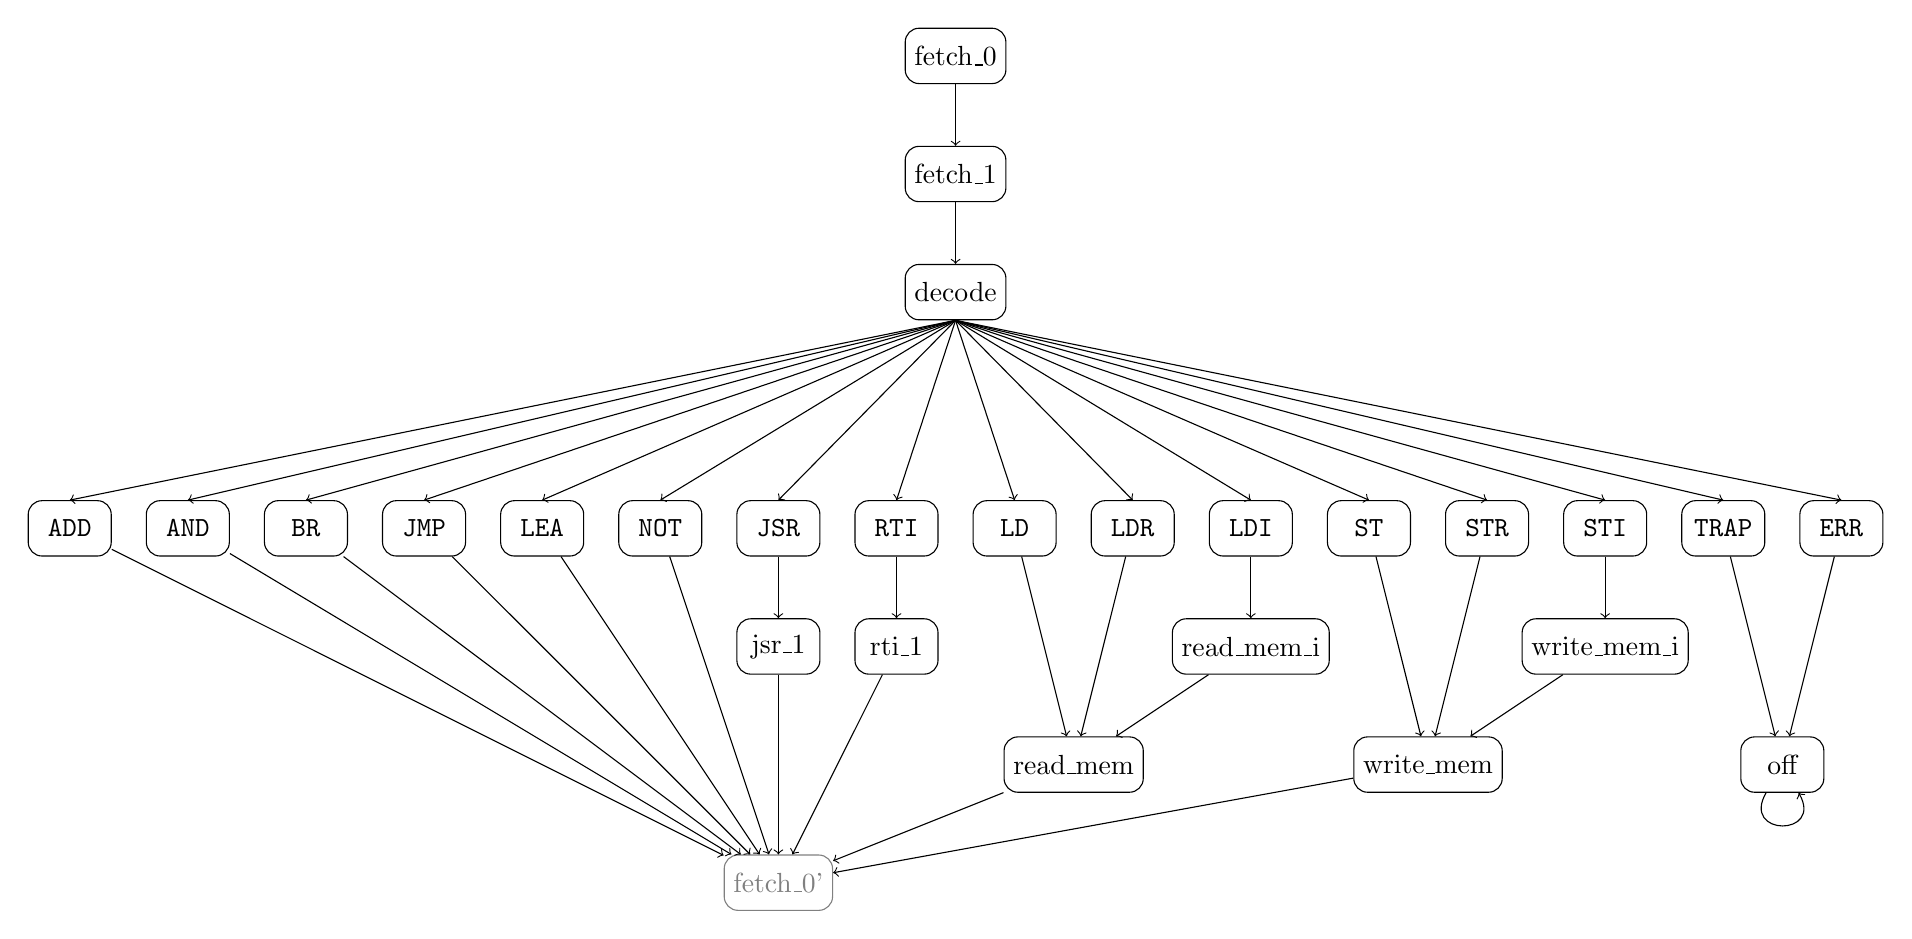
\begin{tikzpicture}[->, align = center, auto, node distance=1.5cm, node/.style = {draw, rectangle, rounded corners =5pt, minimum width =30pt, minimum height =20pt, fill = none}]
      \node[node]                   (fetch0) {fetch\_0};
      \node[node, below of= fetch0] (fetch1) {fetch\_1};
      \node[node, below of= fetch1] (decode) {decode};
      \node[left of = decode, node distance = 0.75cm] (idr) {};
      
      \node[node, below of= idr, node distance = 3cm]    (rti)    {\texttt{RTI}};
      \node[node, left of= rti]     (jsr)    {\texttt{JSR}};
      \node[node, left of= jsr]     (not)    {\texttt{NOT}};
      \node[node, left of= not]     (lea)    {\texttt{LEA}};
      \node[node, left of= lea]     (jmp)    {\texttt{JMP}};
      \node[node, left of= jmp]     (br)     {\texttt{BR}};
      \node[node, left of= br]      (and)    {\texttt{AND}};
      \node[node, left of= and]     (add)    {\texttt{ADD}};
      \node[node, right of= rti]    (ld)     {\texttt{LD}};
      \node[node, right of= ld]     (ldr)    {\texttt{LDR}};
      \node[node, right of= ldr]    (ldi)    {\texttt{LDI}};
      \node[node, right of= ldi]    (st)     {\texttt{ST}};
      \node[node, right of= st]     (str)    {\texttt{STR}};
      \node[node, right of= str]    (sti)    {\texttt{STI}};
      \node[node, right of= sti]    (trap)   {\texttt{TRAP}};
      \node[node, right of= trap]   (err)    {\texttt{ERR}};

      \node[node, below of= jsr]    (jsr1)   {jsr\_1}; 
      \node[node, below of= rti]    (rti1)   {rti\_1};
      \node[below of= decode, node distance = 6cm](ri){};
      \node[node, right of= ri]     (rmem)   {read\_mem};
      \node[node, below of= ldi]    (rmemi)  {read\_mem\_i};
      \node[node, right of= rmem, node distance = 4.5cm] (wmem) {write\_mem};
      \node[node, below of= sti]   (wmemi)  {write\_mem\_i};
      \node[node, right of= wmem, node distance = 4.5cm] (off) {off};
      \node[node, below of= jsr1, node distance = 3cm, draw = gray] (fetch01) {\textcolor{gray}{fetch\_0'}};

      \path[]
      (fetch0) edge (fetch1)
      (fetch1) edge (decode)
      (decode) edge [in = 90, out = 270, looseness = 0] (rti)
      (decode) edge [in = 90, out = 270, looseness = 0] (jsr)
      (decode) edge [in = 90, out = 270, looseness = 0] (not)
      (decode) edge [in = 90, out = 270, looseness = 0] (lea)
      (decode) edge [in = 90, out = 270, looseness = 0] (jmp)
      (decode) edge [in = 90, out = 270, looseness = 0] (br)
      (decode) edge [in = 90, out = 270, looseness = 0] (and)
      (decode) edge [in = 90, out = 270, looseness = 0] (add)
      (decode) edge [in = 90, out = 270, looseness = 0] (ld)
      (decode) edge [in = 90, out = 270, looseness = 0] (ldr)
      (decode) edge [in = 90, out = 270, looseness = 0] (ldi)
      (decode) edge [in = 90, out = 270, looseness = 0] (st)
      (decode) edge [in = 90, out = 270, looseness = 0] (str)
      (decode) edge [in = 90, out = 270, looseness = 0] (sti)
      (decode) edge [in = 90, out = 270, looseness = 0] (trap)
      (decode) edge [in = 90, out = 270, looseness = 0] (err)
      (rti)    edge (rti1)
      (jsr)    edge (jsr1)
      (ld)     edge (rmem)
      (ldr)    edge (rmem)
      (ldi)    edge (rmemi)
      (st)     edge (wmem)
      (str)    edge (wmem)
      (sti)    edge (wmemi)
      (trap)   edge (off)
      (err)    edge (off)
      (off)    edge [out = 240, in = 300, looseness = 4] (off)
      (add)    edge (fetch01)
      (and)    edge (fetch01)
      (br)     edge (fetch01)
      (jmp)    edge (fetch01)
      (lea)    edge (fetch01)
      (not)    edge (fetch01)
      (jsr1)   edge (fetch01)
      (rti1)   edge (fetch01)
      (rmemi)  edge (rmem)
      (wmemi)  edge (wmem)
      (rmem)   edge (fetch01)
      (wmem)   edge (fetch01);
    \end{tikzpicture}
  }
  \label{Fig:fsm}
  \caption{简化后的状态转移图}
\end{figure}

对于在执行过程 (除去 fetch 和 decode) 中只有一个状态的指令, 如 \texttt{ADD, AND}, 其在执行过程的操作与表 \ref{Tab:isa} 中无异.
而其他状态的操作如下表 \ref{Tab:op} 所示.
\begin{table}[!htbp]
  \centering
  \caption{部分状态的操作}
  \label{Tab:op}
  \begin{tabular}{ll}
    \toprule
    状态 & 操作 \\
    \midrule
    fetch\_0 & MAR <- PC, PC <- PC + 1, 刷新寄存器缓冲\\
    fetch\_1 & IR <- MDR, 刷新 PC 缓冲\\
    decode   & 根据 IR 高 4 位确定下一状态\\
    \texttt{RTI} & MAR <- R6, R6 <- R6 + 2\\
    rti\_i & PC <- MDR\\
    \texttt{JSR} & temp <- PC, PC <- PC + PCoffset11 或 BaseR\\
    jsr\_i & R7 <- temp\\
    \texttt{LD} & MAR <- PC + PCoffset9\\
    \texttt{LDR} & MAR <- BaseR + offset6\\
    \texttt{LDI} & MAR <- PC + PCoffset9\\
    read\_mem\_i & MDR <- MDR\\
    read\_mem & DR <- MDR\\
    \texttt{ST} & MDR <- DR, MAR <- PC + PCoffset9, mem\_we <- 1\\
    \texttt{STR} & MDR <- DR, MAR <- BaseR + offset6, mem\_we <- 1\\
    \texttt{STI} & MAR <- PC + PCoffset9, mem\_we <- 0\\
    write\_mem\_i & MAR <- MDR, MDR <- DR, mem\_we <- 1\\
    write\_mem & mem\_we <- 0\\
    \bottomrule
  \end{tabular}
\end{table}

实际上 MDR 由 MDR\_in 和 MDR\_out 组成, 上面的 MDR 只是一个统称.

\subsection*{其他设计细节}
\subsubsection*{内存}
上面提到了在本次实验中使用 IP 核生成了一个 $4096\times16$ bits 的 Single Port RAM, IP 核的设计界面如图 \ref{Fig:ip}. 而内存的实际接线情况见代码 \ref{Code:mem}.
\begin{lstlisting}[style = verilogstyle, caption = 内存的实际接线情况, label = Code:mem]
reg  [15:0] MAR, MDR_in;
reg  mem_we;
wire [15:0] MDR_out;
wire [11:0] MAR12;
initial mem_we <= 1'b0;
assign MAR12 = MAR[11:0];
memory mem(.a(MAR12), 
           .d(MDR_in), 
           .spo(MDR_out), 
           .we(mem_we), 
           .clk(clk_100mhz));
\end{lstlisting}
\img{.8}{images/ip.jpg}{IP 核设计界面}{Fig:ip}
\subsubsection*{状态机编码}
状态机总共 25 个状态, 状态编码共 5 位, 其中指令的编码为 0 + 操作码, 其他状态的编码则为 1xxxx. 这样, 在 decode 阶段, 只需要将 \texttt{\{1'b0,IR[15:12]\}} 赋值给下一阶段即可. 具体的状态机细节可见详细代码 \ref{Code:Source}.
\subsubsection*{条件码 Conditional Code}
条件码用于指示指令的执行结果的正负性, 在本次实验中仅与寄存器类型的 \texttt{result} 有关, 在会改变条件码的指令周期的最后一个状态, 执行结果会被赋值给 \texttt{result} 寄存器, 然后通过以下的组合逻辑电路 (代码 \ref{Code:cc}) 赋值给 \texttt{cc} 寄存器.
\begin{lstlisting}[style = verilogstyle, caption = 条件码的组合逻辑, label = Code:cc]
reg  [15:0] result;
wire [2:0]  cc;
assign cc = (result == 16'h0000) ? 3'b010 : 
              ((result[15] == 1'b0) ? 3'b001 : 3'b100); // setCC
\end{lstlisting}

\subsubsection*{寄存器缓冲}
为了避免在时序逻辑电路的赋值中可能的自赋值冲突的情况 (比如 \texttt{ADD R0, R0, R0} 指令以及 PC 加上偏移的情况), 在本次实验中设计了缓冲, 包括寄存器缓冲 \texttt{R\_buffer} 和 PC 缓冲 \texttt{PC\_buffer}. 其中 \texttt{R\_buffer} 在 fetch\_0 状态刷新 (\texttt{R\_buffer <- R}), 而 \texttt{PC\_buffer} 在 fetch\_1 状态刷新 (\texttt{PC <- PC\_buffer}).
\subsubsection*{I/O}
本次实验用到了四个 sw 开关, 一个 btn 按钮作为输入, 四个七位数码管作为输出. 其中 sw 控制数码管显示的值, 而 btn 则控制着程序的启动. 在比特流文件烧入至 FPGAOL 平台后, LC-3 并不会马上启动, 而是需要按下 btn 后才能开始运行示例程序. 而 sw 的值与七位数码管显示的值的关系如下代码 \ref{Code:sw}.
\begin{lstlisting}[style = verilogstyle, caption = sw 与 hexplay 的关系, label = Code:sw]
  always @(posedge clk_100mhz) begin
  case(sw)
      4'h0: data <= R[0];
      4'h1: data <= R[1];
      4'h2: data <= R[2];
      4'h3: data <= R[3];
      4'h4: data <= R[4];
      4'h5: data <= R[5];
      4'h6: data <= R[6];
      4'h7: data <= R[7];
      4'h8: data <= {7'h00, cc[2], 3'h0, cc[1], 3'h0, cc[0]};
      4'h9: data <= PC;
      4'hA: data <= IR;
      4'hB: data <= MAR;
      4'hC: data <= MDR_out;
      default: data <= 16'h0000;
  endcase
end
\end{lstlisting}

\subsection*{运行示例程序}
前面提到我们将代码 \ref{Code:asm} 的程序导入到了内存中, 该程序的功能实际上是 \texttt{R7 <- R0 * R1}, 将寄存器初值设为 \texttt{\{3, 4, 0, 0, 0, 0, 0, 0\}}, 生成比特流并烧写至 FPGAOL 平台, 系统运行前后的输出如图 \ref{Fig:fpga} 所示. 可以看到在 \ref{Fig:fpga:3} 中, 程序运行完后 R7 的值为 \texttt{x000C}, 符合预期.

\begin{figure}
  \centering
  \subimg{运行前的 R0}{.75}{images/fpga1.jpg}{Fig:fpga:1}
  \subimg{运行前的 R1}{.75}{images/fpga2.jpg}{Fig:fpga:2}
  \subimg{运行后的 R7}{.75}{images/fpga3.jpg}{Fig:fpga:3}
  \caption{运行前后的寄存器状态}
  \label{Fig:fpga}
\end{figure}
\newpage
\subsection*{源代码}
不考虑模拟文件, 整个项目总共有两个文件, 分别是 LC-3 的模块文件与约束文件. 模块文件如代码 \ref{Code:Source}, 约束文件如代码 \ref{Code:Constraint}.
\begin{lstlisting}[style = verilogstyle, caption = 模块文件源代码, label = Code:Source, breaklines = true]
// LC-3.srcs/sources_1/new/main.v
module main(
    input clk_100mhz, btn,
    input [3:0] sw,
    output reg [1:0] hexplay_an,
    output reg [3:0] hexplay_data
    );
// Control LC-3 clock
reg run;
initial run <= 1'b0;
always @(posedge clk_100mhz) if (btn) run <= 1'b1;
// MEMORY
reg [15:0] MAR, MDR_in;
wire [15:0] MDR_out;
wire [11:0] MAR12;
reg mem_we;
initial mem_we <= 1'b0;
assign MAR12 = MAR[11:0];
memory mem(.a(MAR12), 
            .d(MDR_in), 
            .spo(MDR_out), 
            .we(mem_we), 
            .clk(clk_100mhz));
// Finite State Machine
    // control unit
    reg [15:0] PC, IR, PC_buffer;
    initial begin
        PC <= 16'h0000;
        IR <= 16'h0000;
        PC_buffer <= 16'h0000;
    end
    // states
        reg [4:0] curr_state, next_state;
        
        // instruction code, the state is 0+opcode
        
        // Add: DR = SR1 + SR2 or DR = SR1 + imm5
        parameter ADD  = 5'b00001;
        // And: DR = SR1 & SR2 or DR = SR1 & imm5 
        parameter AND  = 5'b00101;
        // Branch: if CC(condition code) meet the
        // requirement the change PC
        parameter BR   = 5'b00000; 
        // Jump: PC = BaseR
        parameter JMP  = 5'b01100;
        // Jump to SubRoutine: Call a subroutine
        // temp = PC
        // then PC = BaseR or PC += PCoffset11
        // then R[7] = temp
        parameter JSR  = 5'b00100;
        // Load: DR = mem[PC + PCoffset9]
        parameter LD   = 5'b00010;
        // Load Indirect: 
        // DR = mem[mem[PC + PCoffset9]]
        parameter LDI  = 5'b01010;
        // Load Base+offset:
        // DR = mem[BaseR + offset6]
        parameter LDR  = 5'b00110;
        // Load Effective Address:
        // DR = PC + PCoffset9
        parameter LEA  = 5'b01110;
        // Not: DR = ~ SR
        parameter NOT  = 5'b01001;
        // Return from Trap or Interrupt
        // (Not effctive since we won't use TRAP
        // except TRAP x25(HALT))
        parameter RTI  = 5'b01000;
        // Store: mem[PC + PCoffset9] = SR(DR here)
        parameter ST   = 5'b00011;
        // Store Indirect: 
        // mem[mem[PC + PCoffset9]] = SR(DR here)
        parameter STI  = 5'b01011;
        // Store Base+offset: 
        // mem[BaseR + offset6] = SR(DR here)
        parameter STR  = 5'b00111;
        // System call:
        // treated as HALT, stop the system
        parameter TRAP = 5'b01111;
        // Error Instrution
        parameter ERR  = 5'b01101;
        
        // instruction cycle phrases and indirect state
        
        // System is off
        parameter off         = 5'h10;
        // Fetch the instructions
        // IR = mem[PC], PC = PC + 1
        parameter fetch_0     = 5'h11;
        parameter fetch_1     = 5'h12;
        // Decode IR to the corresponding state
        parameter decode      = 5'h13;
        // Access the memory
        parameter read_mem    = 5'h14;
        parameter write_mem   = 5'h15;
        parameter read_mem_i  = 5'h16;
        parameter write_mem_i = 5'h17;
        // transfering state
        parameter jsr_1       = 5'h18;
        parameter rti_1       = 5'h19;
        
        initial curr_state <= fetch_0;
    // FSM Part 1
    always @(posedge clk_100mhz) begin
        case (curr_state)
            fetch_0:     next_state <= fetch_1;
            fetch_1:     next_state <= decode;
            decode:      next_state <= {1'b0, IR[15:12]};
            ADD:         next_state <= fetch_0;
            AND:         next_state <= fetch_0;
            BR:          next_state <= fetch_0;
            JMP:         next_state <= fetch_0;
            JSR:         next_state <= jsr_1;
            LD:          next_state <= read_mem;
            LDI:         next_state <= read_mem_i;
            LDR:         next_state <= read_mem;
            LEA:         next_state <= fetch_0;
            NOT:         next_state <= fetch_0;
            RTI:         next_state <= rti_1;
            ST:          next_state <= write_mem;
            STI:         next_state <= write_mem_i;
            STR:         next_state <= write_mem;
            TRAP:        next_state <= off;
            ERR:         next_state <= off;
            read_mem:    next_state <= fetch_0;
            write_mem:   next_state <= fetch_0;
            read_mem_i:  next_state <= read_mem;
            write_mem_i: next_state <= write_mem;
            jsr_1:       next_state <= fetch_0;
            rti_1:       next_state <= fetch_0;
            off:         next_state <= off;
            default:     next_state <= off;
        endcase
    end
    // FSM Part 2 (Processing Unit)
    reg  [15:0] R_buffer [7:0], R [7:0], result, temp;
    wire [2:0]  cc, dr, sr1, sr2, baseR;
    wire [15:0] imm5, PCoffset9, PCoffset11, offset6; // the numbers in the end of instruction after sign-extension
    assign cc         = (result == 16'h0000) ? 3'b010 : ((result[15] == 1'b0) ? 3'b001 : 3'b100); // setCC
    assign dr         = IR[11:9];
    assign sr1        = IR[8:6];
    assign sr2        = IR[2:0];
    assign baseR      = IR[8:6];
    assign imm5       = {{11{IR[4]}}, IR[4:0]};
    assign PCoffset9  = {{7{IR[8]}} , IR[8:0]};
    assign PCoffset11 = {{5{IR[10]}}, IR[10:0]};
    assign offset6    = {{10{IR[5]}}, IR[5:0]};
    initial begin
        R[0]   <= 16'h0004;
        R[1]   <= 16'h0003;
        R[2]   <= 16'h0000;
        R[3]   <= 16'h0000;
        R[4]   <= 16'h0000;
        R[5]   <= 16'h0000;
        R[6]   <= 16'h0000;
        R[7]   <= 16'h0000;
        result <= 16'h0000;
        temp   <= 16'h0000;
    end
    always @(posedge clk_100mhz) begin
        if (run) begin
            case (curr_state)
                fetch_0:begin
                            // Access the memory
                            MAR <= PC_buffer;
                            PC  <= PC_buffer + 16'h0001;
                            // Refresh register buffer
                            R_buffer[0] <= R[0];
                            R_buffer[1] <= R[1];
                            R_buffer[2] <= R[2];
                            R_buffer[3] <= R[3];
                            R_buffer[4] <= R[4];
                            R_buffer[5] <= R[5];
                            R_buffer[6] <= R[6];
                            R_buffer[7] <= R[7];
                            curr_state <= next_state;
                        end
                fetch_1:begin
                            // Load the instruction
                            IR   <= MDR_out;
                            // Refresh PC buffer
                            temp <= PC;
                            PC_buffer <= PC;
                            curr_state <= next_state;
                        end
                ADD: begin // Add: DR = SR1 + SR2 or DR = SR1 + imm5
                         if (IR[5]) begin
                             R[dr]  <= R_buffer[sr1] + imm5;
                             result <= R_buffer[sr1] + imm5;
                         end else begin
                             R[dr]  <= R_buffer[sr1] + R_buffer[sr2];
                             result <= R_buffer[sr1] + R_buffer[sr2];
                         end
                         curr_state <= next_state;
                     end
                AND: begin // And: DR = SR1 & SR2 or DR = SR1 & imm5 
                         if (IR[5]) begin
                             R[dr]  <= R_buffer[sr1] & imm5;
                             result <= R_buffer[sr1] & imm5;
                         end else begin
                             R[dr]  <= R_buffer[sr1] & R_buffer[sr2];
                             result <= R_buffer[sr1] & R_buffer[sr2];
                         end
                         curr_state <= next_state;
                     end
                BR:  begin // Branch: if CC(condition code) meet the
                           // requirement the change PC
                         if (cc & IR[11:9]) PC_buffer <= PC + PCoffset9;
                         curr_state <= next_state;
                     end
                JMP: begin // Jump: PC = BaseR
                         PC_buffer <= R_buffer[baseR];
                         curr_state <= next_state;
                     end
                JSR: begin // Jump to SubRoutine: Call a subroutine
                           // temp = PC
                           // then PC = BaseR or PC += PCoffset11
                           // then R[7] = temp
                         temp <= PC;
                         if (IR[11]) PC_buffer <= PC + PCoffset11;
                         else        PC_buffer <= R_buffer[baseR];
                         curr_state <= next_state;
                     end
                LD:  begin // Load: DR = mem[PC + PCoffset9]
                         MAR <= PC + PCoffset9;
                         curr_state <= next_state;
                     end
                LDI: begin // Load Indirect: 
                           // DR = mem[mem[PC + PCoffset9]]
                         MAR <= PC + PCoffset9;
                         curr_state <= next_state;
                     end
                LDR: begin // Load Base+offset:
                           // DR = mem[BaseR + offset6]
                         MAR <= R_buffer[baseR] + offset6;
                         curr_state <= next_state;
                     end
                LEA: begin // Load Effective Address:
                           // DR = PC + PCoffset9
                         R[dr] <= PC + PCoffset9;
                         curr_state <= next_state;
                     end
                NOT: begin // Not: DR = ~ SR
                         R[dr]  <= ~R_buffer[sr1];
                         result <= ~R_buffer[sr1];
                         curr_state <= next_state;
                     end
                RTI: begin // Return from Trap or Interrupt
                           // (Not effctive since we won't use TRAP
                           // except TRAP x25(HALT))
                         MAR  <= R_buffer[6];
                         R[6] <= R_buffer[6] + 16'h0002;
                         curr_state <= next_state;
                     end
                ST:  begin // Store: mem[PC + PCoffset9] = SR(DR here)
                         MAR    <= PC + PCoffset9;
                         MDR_in <= R_buffer[dr];
                         mem_we <= 1'b1;
                         curr_state <= next_state;
                     end
                STI: begin // Store Indirect: 
                           // mem[mem[PC + PCoffset9]] = SR(DR here)
                         MAR    <= PC + PCoffset9;
                         mem_we <= 1'b0;
                         curr_state <= write_mem_i;
                     end
                STR: begin // Store Base+offset: 
                           // mem[BaseR + offset6] = SR(DR here)
                         MAR    <= R_buffer[baseR] + offset6;
                         MDR_in <= R_buffer[dr];
                         mem_we <= 1'b1;
                         curr_state <= next_state;
                     end
                read_mem:   begin 
                                R[dr]  <= MDR_out;
                                result <= MDR_out;
                                curr_state <= next_state;
                            end
                write_mem:  begin 
                                mem_we <= 1'b0;
                                curr_state <= next_state;
                            end
                read_mem_i: begin
                                MAR <= MDR_out; 
                                curr_state <= next_state;
                            end
                write_mem_i:begin
                                MAR    <= MDR_out;
                                MDR_in <= R_buffer[dr];
                                mem_we <= 1'b1;
                                curr_state <= next_state;
                            end
                jsr_1:   begin
                               R[7] <= temp;
                               curr_state <= next_state;
                         end
                rti_1:   begin
                               PC_buffer  <= MDR_out;
                               curr_state <= next_state;
                         end
                off:     begin
                               mem_we <= 1'b0;
                               curr_state <= next_state;
                         end
                default: curr_state <= next_state;
            endcase 
        end
    end
    // FSM Part 3 (Hexplay)
    reg [18:0] pluse_cnt;
    reg [16:0] data;
    wire pluse_200hz;
    assign pluse_200hz = pluse_cnt == 1'b1;
    always @(posedge clk_100mhz) begin
        if (pluse_cnt >= 19'h7A120) pluse_cnt <= 19'h00000;
        else                        pluse_cnt <= pluse_cnt + 19'h0001;
    end
    always @(posedge clk_100mhz) begin
        if (pluse_200hz) hexplay_an <= hexplay_an + 2'b01;
    end
    always @(posedge clk_100mhz) begin
        case(sw)
            4'h0: data <= R[0];
            4'h1: data <= R[1];
            4'h2: data <= R[2];
            4'h3: data <= R[3];
            4'h4: data <= R[4];
            4'h5: data <= R[5];
            4'h6: data <= R[6];
            4'h7: data <= R[7];
            4'h8: data <= {7'h00, cc[2], 3'h0, cc[1], 3'h0, cc[0]};
            4'h9: data <= PC;
            4'hA: data <= IR;
            4'hB: data <= MAR;
            4'hC: data <= MDR_out;
            default: data <= 16'h0000;
        endcase
    end
    always @(posedge clk_100mhz) begin
        case(hexplay_an)
            2'b00:   hexplay_data <= data[3:0];
            2'b01:   hexplay_data <= data[7:4];
            2'b10:   hexplay_data <= data[11:8];
            2'b11:   hexplay_data <= data[15:12];
            default: hexplay_data <= 4'h0;
        endcase
    end
endmodule
\end{lstlisting}
\begin{lstlisting}[basicstyle = \footnotesize\ttfamily, breaklines=true, numbers = left, language = XML, frame=lrtb, frameround=tttt, caption={约束文件}, label=Code:Constraint]
## LC-3.srcs/constrs_1/new/fpga.xdc

## Clock signal
set_property -dict { PACKAGE_PIN E3    IOSTANDARD LVCMOS33 } [get_ports { clk_100mhz }];

## FPGAOL SWITCH

set_property -dict { PACKAGE_PIN D14   IOSTANDARD LVCMOS33 } [get_ports { sw[0] }];
set_property -dict { PACKAGE_PIN F16   IOSTANDARD LVCMOS33 } [get_ports { sw[1] }];
set_property -dict { PACKAGE_PIN G16   IOSTANDARD LVCMOS33 } [get_ports { sw[2] }];
set_property -dict { PACKAGE_PIN H14   IOSTANDARD LVCMOS33 } [get_ports { sw[3] }];

## FPGAOL HEXPLAY

set_property -dict { PACKAGE_PIN A14   IOSTANDARD LVCMOS33 } [get_ports { hexplay_data[0] }];
set_property -dict { PACKAGE_PIN A13   IOSTANDARD LVCMOS33 } [get_ports { hexplay_data[1] }];
set_property -dict { PACKAGE_PIN A16   IOSTANDARD LVCMOS33 } [get_ports { hexplay_data[2] }];
set_property -dict { PACKAGE_PIN A15   IOSTANDARD LVCMOS33 } [get_ports { hexplay_data[3] }];
set_property -dict { PACKAGE_PIN B17   IOSTANDARD LVCMOS33 } [get_ports { hexplay_an[0] }];
set_property -dict { PACKAGE_PIN B16   IOSTANDARD LVCMOS33 } [get_ports { hexplay_an[1] }];

## FPGAOL BUTTON & SOFT_CLOCK

set_property -dict { PACKAGE_PIN B18   IOSTANDARD LVCMOS33 } [get_ports { btn }];
\end{lstlisting}
\section*{总结与思考}
%请填写对于本次实验的总结与思考,鼓励填写对于本实验或者本课程的各种建议和吐槽。
\begin{description}
  \item[收获] 了解了如何设计一个较为复杂的系统.
  \item[难易程度] 中等
  \item[任务量] 较多
\end{description}
\centering
最后在此感谢老师和助教的付出, 希望这门课能越办越好!
\end{document}
